%%%%%%%%%%%%%%%%
% $Id: synthesis.tex,v 1.8 2009/09/01 21:33:43 jpc Exp $
% $Log: synthesis.tex,v $
% Revision 1.8  2009/09/01 21:33:43  jpc
% Include patches from Fedora (Chitlesh Goorah) and Naohiko Shimizu.
%
% Revision 1.7  2009/08/26 12:25:16  jpc
% Some more adjustments for LaTeX: no more here.sty, rule thickness put
% after begin{document} for fancyhdr.
%
% Revision 1.6  2009/08/26 11:41:46  jpc
% Replacing fancyheaders by fancyhdr for newer LaTeX's versions.
%
% Revision 1.5  2007/12/26 14:55:23  xtof
% ged rif of old styles
%
% Revision 1.4  2004/10/16 12:52:17  fred
% Erasing the psfig include from the file, changed the font to 10 pt
% instead of 12 (sparing trees and not being payed by the thickness of
% my production) and changing font to charter since I got tired of
% Palatino, sorry Herman!
%
%%%%%%%%%%%%%%%%%%%%%%%%%%%%%%%%%%
\documentclass{article}
\usepackage[dvips]{graphics}
\usepackage[english]{babel}
\usepackage{setspace}
\usepackage{fancybox}
\usepackage{fancyhdr}
\usepackage{float}
\usepackage{graphicx}
%\usepackage{here}
%\usepackage{isolatin1}
\usepackage{charter}
\usepackage{picinpar}
\usepackage{rotate}
\usepackage{subfigure}
\usepackage{sverb}
\usepackage{t1enc}
\usepackage{wrapfig}


\setlength{\topmargin}{0cm}
\setlength{\headheight}{1cm}
\setlength{\textheight}{23cm}
\setlength{\textwidth}{16cm}
\setlength{\oddsidemargin}{0cm}
\setlength{\evensidemargin}{0cm}
\setlength{\columnsep}{0.125in}
\setlength{\columnseprule}{0.5pt}
\setlength{\footskip}{1cm}
\setstretch{1}


%--------------------------------- styles
%--------------------------------
%
% Setting the width of the verbatim parts according to 80 tt chars
% Since it is tt, any char is fine
%
\newlength{\verbatimbox}
\settowidth{\verbatimbox}{\scriptsize\tt
xxxxxxxxxxxxxxxxxxxxxxxxxxxxxxxxxxxxxxxxxxxxxxxxxxxxxxxxxxxxxxxxxxxxxxxxxxxxxxxx
}

\newenvironment{sourcelisting}
  {\VerbatimEnvironment\par\noindent\scriptsize
   \begin{Sbox}\begin{minipage}{\verbatimbox}\begin{Verbatim}}%
  {\end{Verbatim}\end{minipage}\end{Sbox}

\setlength{\fboxsep}{3mm}\center\shadowbox{\TheSbox}\normalsize\par\noindent}

\newenvironment{commandline}
  {\VerbatimEnvironment\par\vspace*{2mm}\noindent\footnotesize
   \begin{Sbox}\begin{minipage}{.979\textwidth}\begin{Verbatim}}%
  {\end{Verbatim}\end{minipage}\end{Sbox}\setlength{\shadowsize}{2pt}%
  \shadowbox{\TheSbox}\normalsize\par\noindent}

\pagestyle{fancy}
\rhead{Logic synthesis}
\lhead{PART 2}
\rfoot{\thepage}
\lfoot{ALLIANCE TUTORIAL}
\cfoot{}

%---------------------------------- document ---------------------------------
\begin{document}
\setlength{\footrulewidth}{0.6pt}

\title{
               {\Huge ALLIANCE TUTORIAL\\}
    {\large
               Pierre \& Marie Curie University \\
                       2001 - 2004\\
    }
    \vspace{1cm}
    {\huge
                      PART 2\\
            Logic synthesis
    }
}
\date{}   
\author{
              Ak Frederic\hspace{2cm} Lam Kai-shing\\
Modified by LJ
}

\maketitle

\begin{figure}[H]\centering
  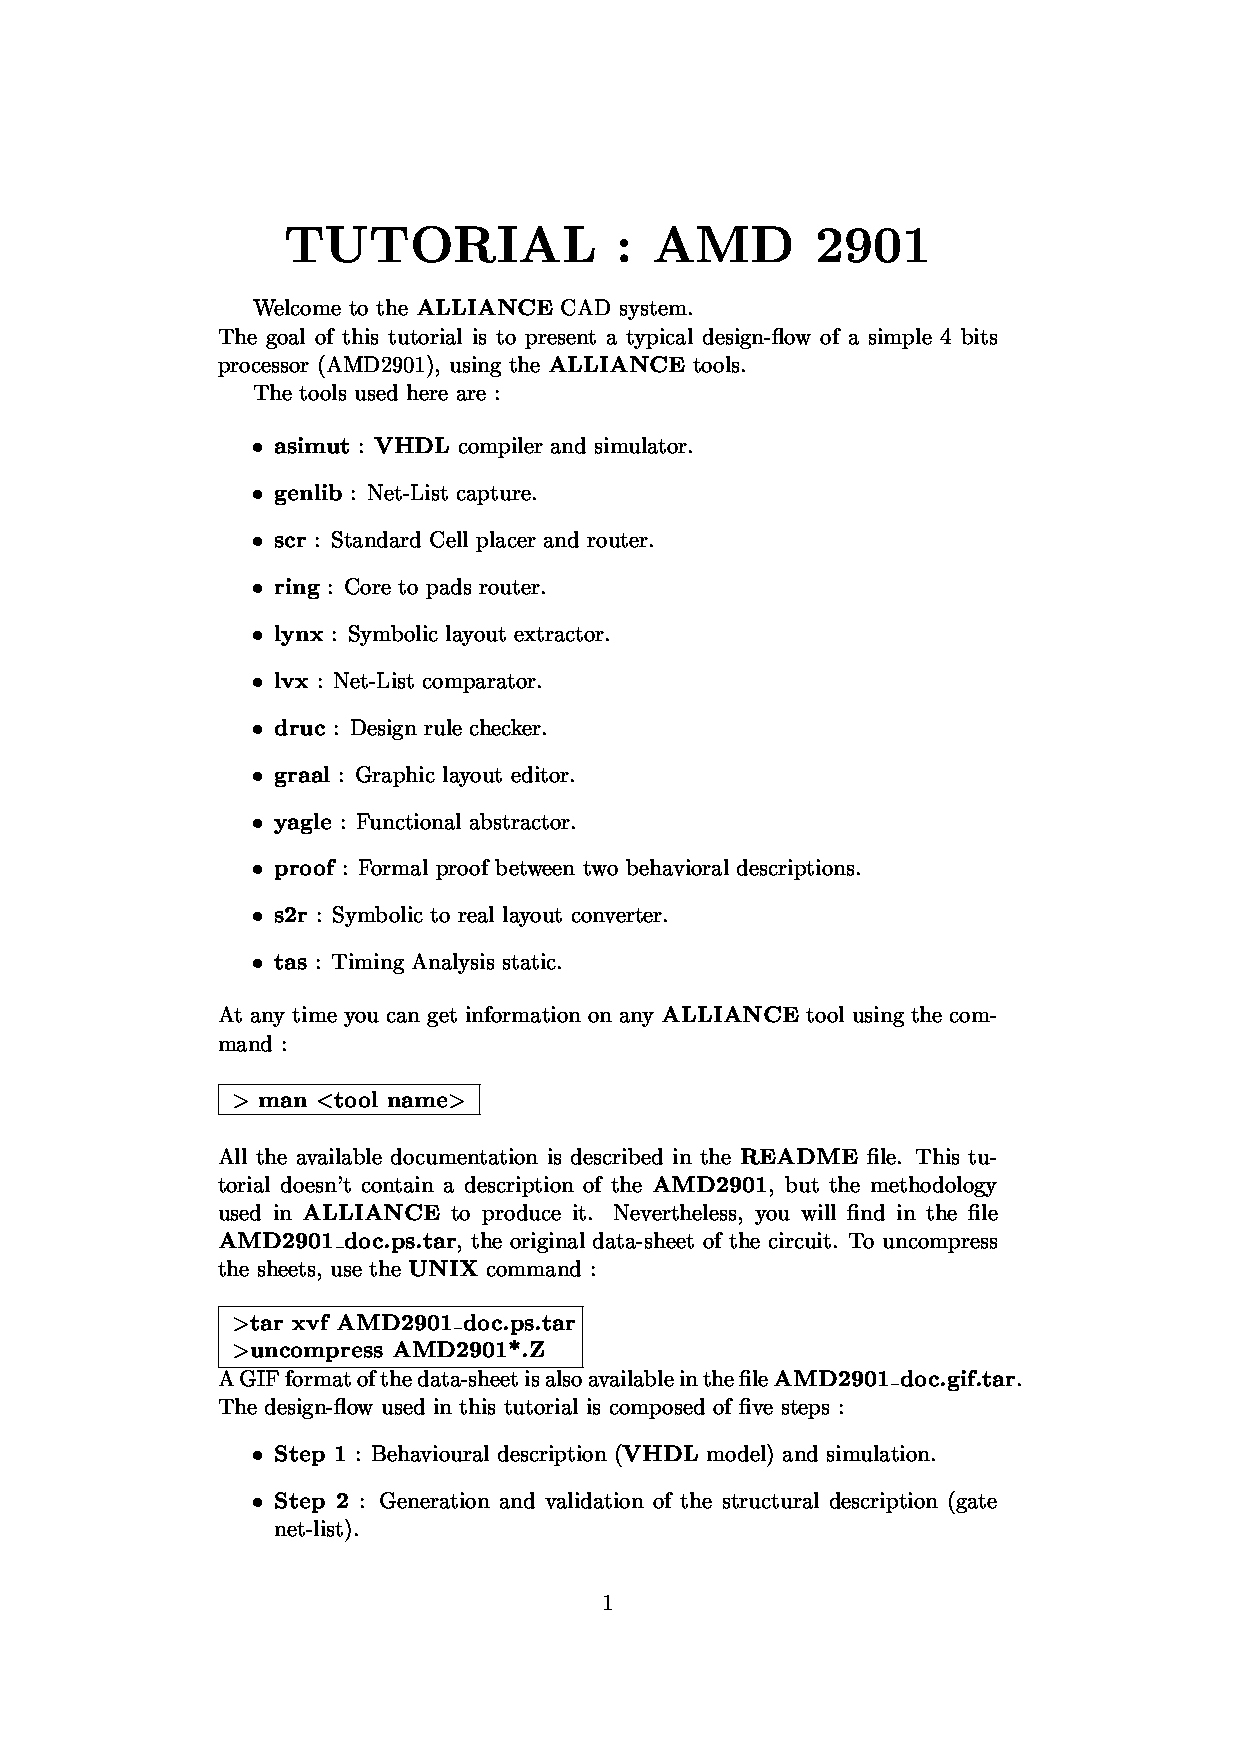
\includegraphics[height=7cm]{amd2901.epsi}
\end{figure}

\begin{figure}
\end{figure}

\thispagestyle{empty}
\def\myfbox#1{\vspace*{3mm}\fbox{#1}\vspace{3mm}}

\newpage
\large{ The purpose of this tutorial is to provide a quick turn of some { \bf
ALLIANCE } tools, developed at the LIP6 laboratory of Pierre and Marie Curie
University.

The tutorial is composed of 3 main parts independent from each other:

\begin{itemize}\itemsep=-.8ex
\item {VHDL modeling and simulation}
\item {Logic synthesis}
\item {Place and route}
\end{itemize}

Before going further you must ensure that all the environment variables are
properly set (source alcenv.sh or alcenv.csh file)
and that the Alliance tools are available when invoking them at the shell
prompt.

All tools used in this tutorial are documented at least with a
manual page.

\newpage
{\bf Contents}\\
\\
 {1} {\bf Introduction}
\\
 {2} {\bf Finite states machine Synthesis}

 {2.1} Introduction

 {2.2} MOORE and MEALY automatons

 {2.3} SYF and VHDL

 {2.4} Example

 {2.5} Step to follow
\\
 {3} {\bf Automat for digicode}

 {3.1} Step to follow
\\
 {4} {\bf Logic synthesis and structural optimization}

 {4.1} Introduction

\hspace{0.5cm} {4.1.1} Logic synthesis

\hspace{0.5cm} {4.1.2} Solve fan-out problems 

\hspace{0.5cm} {4.1.3} Long path visualization 

\hspace{0.5cm} {4.1.4} Netlist Checking

\hspace{0.5cm} {4.1.5} Scan-path insertion

 {4.2} Step to follow

\hspace{0.5cm} {4.2.1} {\it Mapping} on predefined cells

\hspace{0.5cm} {4.2.2} Netlist visualization

\hspace{0.5cm} {4.2.3} Boolean network optimization

\hspace{0.5cm} {4.2.4} Netlist optimization 

\hspace{0.5cm} {4.2.5} Netlist checking

\hspace{0.5cm} {4.2.6} Scan-path insertion in the netlist
\\
 {5} {\bf AMD 2901}

 {5.1} exercise

 {5.2} step to follow

 {5.3} error found
\\
 {6} {\bf AMD2901 structure}
\\
 {7} {\bf Part controls design }

 {7.1}{ \bf genlib } description example 

 {7.2} provided files checking

 {7.3} Part controls description
\\
 {8} {\bf Data-path design}

 {8.1} Example of description with genlib macro-functions

 {8.2} Data-path description
\\
{9} {\bf The { \it Makefile } or how to manage tasks dependency }

 {9.1.1} Rules

 {9.1.2} models Rules

 {9.1.3} Variables definitions 

 {9.1.4} Predefined variables
\\
 {10} {\bf Appendix: Diagrams as an indication but not-in conformity with the behavioral}


\newpage
       {\huge
        PART 2 :\\ }
        \vspace{1cm}
        {\huge
        Logic Synthesis
        }

All the files used in this part are located under \\
\texttt{/usr/share/doc/alliance-doc-5.0/tutorials/synthesis/src} directory.\\
This directory contents four subdirectories and one Makefile :
\begin{itemize}\itemsep=-.8ex

\item   Makefile
\item   amdbug
    \begin{itemize}\itemsep=-.8ex
    \item   Makefile
    \item   amdfindbug.pat : tests file
    \item   several files amd.vbe : behavioral description
    \end{itemize}
\item   counter
    \begin{itemize}\itemsep=-.8ex
    \item   Makefile
    \item   cpt5.fsm : description in fsm
    \item   cpt5.pat : tests file
    \end{itemize}
\item   digicode
    \begin{itemize}\itemsep=-.8ex
    \item   Makefile
    \item   digicode.fsm : description in fsm
    \item   paramfile.lax : use to modify the fan-out
    \item   digicode.pat : tests file
    \item   scan.path : make it possible to observe registers
    contents
    \end{itemize}
\item   amd2901
    \begin{itemize}\itemsep=-.8ex
    \item   Makefile
    \item   amd2901\_ctl.vbe : behavioral description of control
    part
    \item   amd2901\_dpt.vbe : behavioral description of data-path
    \item   amd2901\_ctl.c : file .c of control part
    \item   amd2901\_dpt.c : file .c of data-path
    \item   amd2901\_core.c : file .c of heart
    \item   amd2901\_chip.c : file .c of the circuit with their
    pads
    \item   pattern.pat : tests file
    \end{itemize}
\end{itemize}


\newpage
\section{Introduction}
%---------------------
    The goal of this section is to present some ALLIANCE tools which are:

\begin{itemize}\itemsep=-.8ex
\item   Logic synthesis tools { \bf SYF, BOOM, BOOG, LOON, SCAPIN };
\item   Data-path generation tool{\bf GENLIB };
\item   { \it netlist } graphical viewer  { \bf XSCH };
\item   formal proof Tools {\bf FLATBEH, PROOF};
\item   The simulator { \bf ASIMUT };
\end{itemize}

The first two sections will relate to the { \it netlist } { \bf
generation and validation } methods of predefined cells. Indeed,
even if it is acquired that the tools for ALLIANCE generation
function correctly, the validation of each generated view is { \bf
essential }. It makes it possible to limit
the cost and the time of the design.  \\
The two other sections will be reserved for the { \bf data-path
generation and the control part } of AMD2901.

\section{Finite states machine Synthesis}

\subsection{Introduction}

A pure combinatorial circuit has no internal registers. So
its outputs depend only on its primary inputs. On the contrary 
a synchronous sequential circuit having internal registers sees its
outputs changing according to its inputs but also memorized values
in its registers. As consequence, the circuit state at the moment
t+1 also depends on its state at the moment t. This type of
circuit can be formally modelized as a { \bf finite states machine}.

\begin{figure}[H]\centering
  \includegraphics[width=9cm]{ex_digicode.eps}
 \caption{Automat}
  \label{Fig:ex_digicode}
\end{figure}

\subsection{MOORE and MEALY automaton}
%---------------------------------------
The MOORE automaton sees the state of its outputs changing only on
clock-edges. The inputs can thus move between two clock-edges
without modifying the outputs. But in the case of MEALY automaton,
the variation of the inputs can modify at any time the value of
the outputs. It will be essential to separate the generation
function from the transition function (Moore automaton).
Two distinct processes will then modelize the next state computation
and the current state register update.

\begin{figure}[H]\centering
  \includegraphics[width=15cm]{automate.eps}
 \caption{Automats}
  \label{Fig:automaton}
\end{figure}


\subsection{SYF and VHDL}
%-----------------------
In order to describe the automatons, we use a particular {\bf VHDL }
style description that defines architecture "FSM" ({ \bf
F}inite-{\bf S}tate { \bf M}achine).

The corresponding file also has the extension { \bf fsm }. From
this file, the tool { \bf SYF } makes the automaton synthesis and
after state encoding, it transforms this abstracted automaton into
a Boolean network and a state register. 
{ \bf SYF } then generates a { \bf VHDL } file using the 
{\bf vbe } subset. 
Like most of all tools used in alliance, it is
necessary to set some variables before using { \bf SYF }. 
You can refer to the { \bf man } page of { \bf syf } for more details.

\subsection{Example}
%-------------------

In order to take in hand the particular syntax of a {
\bf fsm } file, an example of { \bf three } successive "1" counter
is presented. Its vocation is to detect for example on a
connection series, a sequence of { \bf three } successive "1" counter.
The state graph is represented on the figure
\ref{Fig:graphe1}.\\
The { \bf fsm } format is detailed in the man page { \bf fsm(5) }.

\begin{sourcelisting}
    entity circuit is
          port (
               ck, i, reset, vdd, vss : in bit;
               o : out bit
          );
    end circuit;
    architecture MOORE of circuit is
          type ETAT  _TYPE is (E0, E1, E2, E3);
          signal EF, EP : ETAT  _TYPE;
- - pragma CURRENT  _STATE EP
- - pragma NEXT  _STATE EF
- - pragma CLOCK CK
    begin
          process (EP, i, reset)
          begin
               if (reset='1') then
                    EF<=E0;
               else
                    case EP is
                         when E0 =
                              if (i='1') then
                                   EF <= E1;
                              else
                                   EF <= E0;
                              end if;
                         when E1 =
                              if (i='1') then
                                   EF <= E2;
                              else
                                   EF <= E0;
                              end if;
                         when E2 =
                              if (i='1') then
                                   EF <= E3;
                              else
                                   EF <= E0;
                              end if;
                         when E3 =
                              if (i='1') then
                                   EF <= E3;
                              else
                                   EF <= E0;
                              end if;
                         when others =  assert ('1')
                              report "etat illegal";
                   end case;
               end if;
               case EP is
                    when E0 =
                         o <= '0' ;
                    when E1 =
                         o <= '0' ;
                    when E2 =
                         o <= '0' ;
                    when E3 =
                         o <= '1' ;
                    when others =  assert ('1')
                         report "etat illegal";
              end case;
          end process;
          process(ck)
          begin
               if (ck='1' and not ck'stable) then
                    EP <= EF;
               end if;
          end process;
    end MOORE;
\end{sourcelisting}

\begin{figure}[H]\centering
 \includegraphics[height=8cm]{graphe1.eps}
 \caption{states graph of three successive "1" counter}
 \label{Fig:graphe1}
\end{figure}


\subsection{Step to follow}
%---------------------------------

Now you can use this example to write the description of a { \bf five } successive "1" 
counter in a{\bf Moore } automaton.

\begin{itemize}\itemsep=-.8ex
\item   position the environment variables . \item   launch { \bf
SYF } with the coding options { \bf -a, -J, -m, -O, -R }
        and by using the options { \bf -CEV }. \ \
       
       -a        Uses "Asp" as encoding algorithm.

       -j        Uses "Jedi" as encoding algorithm.

       -m        Uses "Mustang" as encoding algorithm.

       -o        Uses the one hot encoding algorithm.

       -r        Uses distinct random numbers for state encoding.

\begin{commandline}
> syf -CEV -a <fsm_source>
\end{commandline}
\item   visualize the files { \bf enc }. Those files contains one state
	name followed by its hexadecimal code value.

\item   write stimuli (test vectors) and simulate with { \bf ASIMUT }.
\end{itemize}

%\subsection{Utilisation d'un chemin de test ({\it scan-path}\/)}
%-------------------------------------------------------
%   Pour ins\'erer automatiquement un chemin de scan qui permet
%d'observer en mode test le contenu de tous les registres du circuit, il
%faut ajouter au fichier {\bf .fsm} les commandes suivantes:\\
%
%\begin{itemize}\itemsep=-.8ex
%\item  ajouter les connecteurs n\'ecessaires au {\it scan-path}\/ par exemple:\\
%   \\
%   test    : in bit\\
%   scanin  : in bit\\
%   scanout : out bit\\
%\item ajouter les pragmas n\'ecessaires au {\it scan-path}\/ par exemple:\\
%   \\
%   - -pragma SCAN\_TEST  test\\
%   - -pragma SCAN\_IN  scanin\\
%   - -pragma SCAN\_OUT  scanout
%\item  Choisir un codage et relancer {\bf SYF} avec l'option {\bf -P}
%        qui ajoute le {\it scan-path}\/.
%\item  Ecrire un fichier de vecteurs de test permettant de v\'erifier le
%   fonctionnement du {\it scan-path}\ et simuler sous {\bf ASIMUT}.
%\end{itemize}
%

\newpage

\section{Automaton for digicode}
%-------------------------------

We want to design a digicode circuit whose keyboard is
represented on the figure \ref{Fig:keyboard}. 
The specifications are as follows:

\begin{figure}[H]\centering
  \includegraphics[width=7cm,height=7cm]{clavier.eps}
  \caption{Clavier}
  \label{Fig:keyboard}
\end{figure}

\begin{itemize}\itemsep=-.8ex
\item   The numbers from 0 to 9 are coded in natural binary on 4 bits.
    A and B are coded in the following way:
    \begin{itemize}\itemsep=-.8ex
    \item   A: 1010
    \item   B: 1011
    \end{itemize}
\item   The digicode works in two modes:
    \begin{itemize}\itemsep=-.8ex
    \item   Day Mode: The door opens while pressing on "O" or if entering the good code
    \item   Night Mode: The door opens only if the code is correct.
    \end{itemize}
    To distinguish the two cases an external "timer" calculates the signal { \bf day}
    which is equal to ' 1 ' between 8h00 and 20h00 and ' 0 ' otherwise.
\item   The digicode order an alarm as soon as one of the entered
numbers is not the good. \item   The digicode automaton returns in
idle state if nothing
    returned to the keyboard at the end of 5 seconds
        or if alarm sounded during 2mn - signal { \it \bf reset } -. For that it receives a signal
        from { \bf reset } external timer.
\item   The chip works at 10MHz.
\item   Any pressure of a key of the keyboard is then followed by the signal { \it \bf press\_kbd }.
        This one announces to the chip that the output data of the
        keyboard is valid.  This signal is set to 1 during a clock-edge.
\end{itemize}

The code is { \bf 53A17 } (but you can take the code who agrees to
you). The interface of this automaton is as follows:

\begin{itemize}\itemsep=-.8ex
\item   in {\bf ck}
\item   in {\bf reset}
\item   in {\bf day}
\item   in {\bf i[3:0]}
\item   in {\bf O}
\item   in {\bf press\_kbd}
\item   out {\bf door}
\item   out {\bf alarm}
\end{itemize}


\begin{figure}[H]\centering
 \includegraphics[height=8cm]{graphe_solution_digicode.eps}
 \caption{Digicode states graph}
 \label{Fig:graph 2}
\end{figure}

\subsection{Step to follow}
%---------------------------------

\begin{itemize}\itemsep=-.8ex
\item   draw the states graph.
\item   describe it in the { \bf fsm } format . 
\item   synthesize your description with { \bf SYF } using 
        different state encoding algorithms
       { \bf -a, -j, -m, -o, -r } and by using the options { \bf -CEV}.\\
\begin{commandline}
> syf -CEV -a <fsm_source>
\end{commandline}
\item  write stimuli (test vectors).
\item  simulate with { \bf ASIMUT } all the resulting {\bf vbe} descriptions.
\end{itemize}

\newpage
%%%%%%%%%%%%%%%%%%%%%%%%%%%%%%%%%%%%%%%%%%%%%%%%%%%%%%%%%%%%%

\section{Logic synthesis and structural optimization}
%--------------------------------------------------------

\subsection{Introduction}
%------------------------

\subsubsection{Logic synthesis}
%---------------------------------
    The logic synthesis permits to obtain a { \it netlist } of
    gates given a Boolean network (format { \bf vbe }). 
    Several tools are available:

\begin{itemize}\itemsep=-.8ex
\item  The tool { \bf BOOM } allows the Boolean network optimization before mapping with { \bf BOOG }.
\item  The tool { \bf BOOG } synthesizes a { \it netlist } by using a library
       with predefined cells such as { \bf SXLIB }.
       The { \it netlist } can be either with the format { \bf vst } or with the format { \bf al }.
       Check the environment variable { \bf MBK\_OUT\_LO}=vst.
\end{itemize}\itemsep=-.8ex

\subsubsection{Solve fan-out problems }
%-----------------------------------------------------
    Generated { \it netlist}\/s may contain internal signals that drive a
    significant number of gates (large FAN-OUT).
    In order to solve this problem, the tool
    { \bf LOON } replaces the cells having a too large fan-out by more powerful
    cells and/or insert buffers.

\subsubsection{Long path visualization }
%-----------------------------------------------------
    At any moment, the { \it netlist}\/s can be graphically displayed using {\bf XSCH}.
This tool permits also to highlight the longest path on the schematic thanks to the files { \bf
xsc } and { \bf vst } generated by { \bf BOOG } and { \bf LOON }.

\begin{figure}[H]\centering
  \includegraphics[]{T_RC.eps}
 \caption{Simplified timing diagram }
  \label{Fig:T_RC}
\end{figure}

Equivalent resistor { \it R } of the { \it figure \ref{Fig:T_RC} }
is calculated on the totality of the transistors of the { \it AND
} belonging to the active way. In the same way, the capacity { \it
C } is calculated on the busy transistors of the { \it NOR }
corresponding to the way between { \it i0 } and the output of the
cell.

\subsubsection{Netlist Checking}
%-----------------------------------------------------
    The netlist must be validated. For that, you have { \bf ASIMUT },
    but also the tool { \bf PROOF } which proceeds to a formal comparison of two behavioral
    descriptions ({ \bf vbe }). The tool { \bf FLATBEH } is usefull to obtain a
    new behavioral file starting from a { \it netlist } 
   (given a {\bf vbe} file for each leave cells of the hierarchy).

\subsubsection{Scan-path insertion}
%-----------------------------------------------------
    With { \bf SCAPIN } we can insert a scan-path into the netlist.
    The scan-path allow the designer to observe in test mode the value of all registers of your circuit. 
    The path is created by changing each registers into a mux\_register (or by inserting a multiplexer
    in front of all registers).

\newpage

\subsection{Step to follow}
%---------------------------------

\subsubsection{{\it Mapping} on predefined cells}
%----------------------------------------------------------
    For each Boolean network obtained previously:

\begin{itemize}\itemsep=-.8ex
\item set properly environment variables; 
\item synthesize the structural view:
\begin{commandline}
> boog <vbe_source>
\end{commandline}
\item launch { \bf BOOG } on different {\it netlist}\/s to observe {\bf SYF}
      options influence (different state encoding technics).
\item validate the work of { \bf BOOG } with { \bf ASIMUT }, 
      the { \it netlist}\/s obtained with stimuli which were used to 
      validate the initial Boolean network.
\end{itemize}\itemsep=-.8ex

\subsubsection{Netlist visualization}
%----------------------------------------------------------

\begin{itemize}\itemsep=-.8ex
\item The longest path (critical path) is described in the { \bf xsc } file produced
      by { \bf boog }.
      The { \bf XSCH } tool  will use it to highlight this path on the schematic.
      To launch the graphical schematic viewer:
\begin{commandline}
>xsch -I vst -l <vst_source>
\end{commandline}
\item The red color indicates the critical path.
\item you can use the option '{ \it -slide }' followed by netlist names to display one by one a set of
      schematics.
      The keys ' { \it + } ' and ' { \it - }' can then be used to display respectively next and previous
      netlist.
\end{itemize}\itemsep=-.8ex


\subsubsection{Boolean network optimization}
%-------------------------------------------------
    To analyze Boolean optimization effect :

\begin{itemize}\itemsep=-.8ex
\item   launch Boolean optimization with the tool { \bf BOOM }
        by asking an optimization in { \bf surface } then in { \bf delay } ;
\begin{commandline}
>boom -V <vbe_source> <vbe_destination>
\end{commandline}

\item   test { \bf BOOM } with the various algorithms - S, - J, -
B, - G, - p..., the options specifie which algorithm has to be used for the boolean optimization.
    
\item   compare the literal number after factorization. \item
remake the Boolean networks synthesis with the tool { \bf BOOG }
        and compare the results.
\end{itemize}

\subsubsection{Netlist optimization }
%-------------------
    For all the structural view obtained previously:
\begin{itemize}\itemsep=-.8ex
\item   launch { \bf LOON } with the command:
\begin{commandline}
>loon <vst_source> <vst_destination> <lax_param>
\end{commandline}
\item   carry out an fanout optimization by modifying the fanout
factor in the option file { \bf .lax }.The optimization mode and level are able to be change in this file.
 \item   impose capacities
values on the outputs.
\end{itemize}

\subsubsection{Netlist checking}
%-------------------
    to carry out on the best of your { \it netlist}\/s:

\begin{itemize}\itemsep=-.8ex
\item   validate the work of { \bf LOON } by running { \bf ASIMUT } 
        on the different { \it netlist}\/s obtained, using the stimuli 
        that were defined to validate the initial behavioral view.
\item   Make a formal comparison of your netlist with
        the original behavioral file resulting from { \bf SYF }:
\begin{commandline}
>flatbeh <vst_source> <vbe_dest>
\end{commandline}
\begin{commandline}
>proof -d <vbe_origin> <vbe_dest>
\end{commandline}
\end{itemize}

Checks if the files are formally identicals.

\subsubsection{Scan-path insertion in the netlist}
%-------------------
    to carry out on the best of your { \it netlist}\/s:

\begin{itemize}\itemsep=-.8ex
\item   insert a scan-path connecting all the digicode registers.
\begin{commandline}
>scapin -VRB <vst_source> <path_file> <vst_dest>
\end{commandline}

\newpage

\# Example of .path file
\begin{sourcelisting}
BEGIN_PATH_REG

cs_0
cs_1
cs_2
END_PATH_REG

BEGIN_CONNECTOR

SCAN_IN      scin
SCAN_OUT     scout
SCAN_TEST    test
END_CONNECTOR
\end{sourcelisting}
\item   build ten patterns to test the scan-path and simulate with
{ \bf ASIMUT }.
\end{itemize}\itemsep=-.8ex

\newpage
\section{AMD 2901}

\subsection{exercise}

First of all, here is an exercise to understand the AMD2901
chip functionality. The goal is to design it 
using Alliance, as described in the following parts of
this tutorial.

To explore all functionalities, you will have
to validate the behavioral view that will be provided. 
All needed informations will be find in appendix.

The validation will have to be done using stimuli 
generated by {\bf genpat}. The vectors must be carefully written
to enable you to detect { \bf BUG } in your behavioral file { \bf .vbe }. 
Approximately 500 patterns will be enough for debugging your AMD 2901.

\subsection{step to follow}
It is necessary to generate stimuli that tests all the parts and all functions
of the AMD following the specifications described in the documentation.

\begin{itemize}\itemsep=-.8ex
\item   filling and reading the 16 boxes memories of the RAM .
\item   test the RAM shifter
\item   filling and reading of the accumulator.
\item   test the accumulator shifter .
\item   test the arithmetic and logic operations
        (addition, subtraction, overflow, carry, propagation, etc...) .
\item   exhaustive test of the inputs conditioned by I[2:0].
\item   data-path test vectors
\end{itemize}

\subsection{error found}

You can notice that for the RAM shifter values "101" and "111" of
i[8:6], the AMD causes a shift of the accumulator that should not
take place.

for the values "000" and "001" of i[8:6], the circuit writes the
ALU output in RAM .

The AMD carries out the operation R xor S for
I[5:3]=111 instead of carrying out the operation for I[5:3]=110.

It carries out the operation /(R Xor S) for I[5:3]=110 instead of
I[5:3]=111.

\newpage
\section{AMD2901 structure}


We break up Amd2901 into 2 blocks: %la partie cont\^ole qui regroupe la ``glu'' logique et la partie op\'erative (chemin de donn\'ees).%
\begin{figure}[H]\center
\leavevmode
\includegraphics[width=10cm]{bloc}
\caption{Amd2901 Organization  \label{bloc}}
\end{figure}


\begin{itemize}\itemsep=-.8ex
\item The data-path contains the Amd2901 regular parts , the
registers and the arithmetic logic unit. 
\item The control part contains irregular logic, 
      the instructions decoding and the flags computation.
\end{itemize}

\newpage
We will use the following hierarchical description:
\begin{figure}[H]\center
\leavevmode
\includegraphics[width=10cm]{hier}
\caption{Hierarchy \label{hier}}
\end{figure}

The provided files are as follows:\\
\begin{itemize}\itemsep=-.8ex
\item amd2901\_ctl.vbe, behavioral description of the part
controls \item amd2901\_dpt.vbe, behavioral description of the
part data-path \item amd2901\_ctl.c, file { \bf C } of the part
controls \item amd2901\_dpt.c, file { \bf C } of the part of data
path \item amd2901\_core.c, file { \bf C } of the heart \item
amd2901\_chip.c, file { \bf C } of the circuit containing the pads
\item pattern.pat, tests file \item CATAL, file listing the
behavioral files, to be modify \item Makefile, to automate the
generation
\end{itemize}


%%%%%%%%%%%%%%%%%%%%


\newpage
\section{Part controls design }


This part of irregular logic will be carried out with the cells of the library {\bf SXLIB}.\\
\\
Description in VHDL netlist (i.e { \it .vst }) of the various
gates hazardous when the circuit contain
several thousands of them. there exists a tool for procedural
signals lists generation , { \bf genlib }. It is then enough to
describe in C using macro-functions the { \it signals list } in
gates of the block. The library of macro-functions C is called {
\bf genlib }. The { \bf genlib } execution produces a description
VHDL with the format { \it .VST }. For more details, consult the
manual (man) on { \bf genlib }.

\subsection{{ \bf genlib } description example }

here a simple circuit:

\begin{figure}[H]\center
\leavevmode
\includegraphics[width=10cm]{exemple1}
\end{figure}

The equivalent { \bf genlib } file is as follows:

\begin{sourcelisting}
#include <genlib.h>
    main()
      {
       GENLIB_DEF_LOFIG("circuit");

       /* Connectors declaration */
       GENLIB_LOCON("a",IN,"a1");
       GENLIB_LOCON("b",IN,"b1");
       GENLIB_LOCON("c",IN,"c1");
       GENLIB_LOCON("d",IN,"d1");
       GENLIB_LOCON("e",IN,"e1");
       GENLIB_LOCON("s",OUT,"s1");

       GENLIB_LOCON("vdd",IN,"vdd");
       GENLIB_LOCON("vss",IN,"vss");

       /* Combinatorial gates instanciation */
       GENLIB_LOINS("na2_x1","nand2","a1","c1","f1","vdd","vss",0);
       GENLIB_LOINS("no2_x1","nor2","b1","e1","g1","vdd","vss",0);
       GENLIB_LOINS("o2_x2","or2","d1","f1","h1","vdd","vss",0);
       GENLIB_LOINS("inv_x1","inv","g1","i1","vdd","vss",0);
       GENLIB_LOINS("a2_x2","and2","h1","i1","s1","vdd","vss",0);

       /* Save of the figure */
       GENLIB_SAVE_LOFIG();
       exit(0);
      }
\end{sourcelisting}

Save it under the name `` circuit.c '' then compile the file with
the command : \
\begin{commandline}
> genlib circuit
\end{commandline}

You obtain the file `` circuit.vst ''. (if is not it, it may be
due to environment variables that are not properly set for { \bf genlib }).

\subsection{provided files checking}
Create the file { \bf CATAL } in your simulation directory . It
must contain the following lines:
\ \\
\begin{commandline}
amd2901_ctl C
amd2901_dpt C
\end{commandline}

It makes the simulator use the
behavioral files (.vbe) of `` amd2901\_ctl '' and of `` amd2901\_dpt ' '. \\

\begin{commandline}
> asimut amd2901_chip pattern result
\end{commandline}

You can verify the resulting patterns by using { \bf xpat } on the file ``
result ''.

\subsection{Part controls description }

The diagrams corresponding to the signals list to design are
provided to you. %To supplement the file `` amd2901\_ctl.c '' then
compile it by using the steps below. \\

%Positionner les variables d'environnement sp\'ecifiant les formats des diff\'erentes vues ainsi que les librairies de cellules utilis\'ees.\\
%
%\myfbox{
%\shortstack[l]{
%{\bf $>$ setenv VH\_MAXERR 10}\\
%{\bf $>$ setenv VH\_BEHSFX vbe}\\
%{\bf $>$ setenv VH\_PATSFX pat}\\
%{\bf $>$ setenv VH\_LIBLST .}\\
%{\bf $>$ setenv MBK\_WORK\_LIB .}\\
%{\bf $>$ setenv MBK\_CATA\_LIB .:\$ALLIANCE\_TOP/cells/sxlib:}\\
%{\bf \$ALLIANCE\_TOP/cells/padlib}\\
%{\bf $>$ setenv MBK\_CATAL\_NAME CATAL}\\
%{\bf $>$ setenv MBK\_IN\_LO vst}\\
%{\bf $>$ setenv MBK\_OUT\_LO vst}\\
%{\bf $>$ setenv MBK\_IN\_PH ap}\\
%{\bf $>$ setenv MBK\_OUT\_PH ap}
%}
%}\\

Generate the signals list { \bf vst } starting from the file { \bf
c } by the command:
\begin{commandline}
> genlib amd2901_ctl
\end{commandline}

Then validate the structural view obtained by simulating the
complete circuit with the tests vectors which are provided to you.
Replace the behavioral view of the part controls by his structural
view by removing the name { \it amd2901\_ctl } of { \bf CATAL }
file.

\begin{commandline}
> asimut -zerodelay amd2901_chip vecteurs result
\end{commandline}

Note that one carries out a simulation `` without delay '' of the netlist. In the event
of problem, do not hesitate to use { \bf xpat }.

\begin{commandline}
> asimut amd2901_chip pattern result
\end{commandline}

After having validated the functional behavior of the netlist,
simulate it using propagation delays. 
Modify time values between the patterns. Indeed, {
\bf asimut } is able to evaluate the propagation times for each
cell of the netlist (taken into account the "after" clauses 
specify in vbe files).

%%%%%%%%%%%%%%%%%%%%

\newpage
\section{Data-path design}
The data path is formed by the regular logic of the circuit. In
order to benefit from this regularity, we generates the signals
list in the vectorial operators form (or columns) { \it via } the
macro-functions of the tool { \bf genlib } . That makes it
possible to save place by using several times the same material .
For example, the { \it NOT } of a mux of { \it N } bits is
instanciate only once for these { \it N } bits...

\subsection{Example of description with genlib macro-functions}

Let us consider the following circuit:

\begin{figure}[H]\center
\leavevmode
\includegraphics[width=10cm]{exemple2}
\end{figure}

Here the corresponding data-path structure :
\begin{figure}[H]\center \leavevmode
\includegraphics[width=10cm]{datap}
\end{figure}

Each gate occupies a column, a column making it possible to treat
a whole of bits for the same operator. The first line represents bit 3, the last bit 0 .

\newpage

The file { \bf genlib } correspondent is as follows:

\begin{sourcelisting}
#include <genlib.h>
    main()
      {
       GENLIB_DEF_LOFIG("data_path");

       /* connectors declaration */
       GENLIB_LOCON("a[3:0]",IN,"a[3:0]");
       GENLIB_LOCON("b[3:0]",IN,"b[3:0]");
       GENLIB_LOCON("c[3:0]",IN,"c[3:0]");
       GENLIB_LOCON("v",IN,"w");
       GENLIB_LOCON("cout",OUT,"ct");
       GENLIB_LOCON("s[3:0]",OUT,"s[3:0]");
       GENLIB_LOCON("cmd",IN,"cmd");
       GENLIB_LOCON("vdd",IN,"vdd");
       GENLIB_LOCON("vss",IN,"vss");

       /* operators creation */
       GENLIB_MACRO(GEN_NAND2, "model_nand2_4bits", F_PLACE, 4, 1);
       GENLIB_MACRO(GEN_OR2, "model_or2_4bits", F_PLACE, 4);
       GENLIB_MACRO(GEN_ADSB2F, "model_add2_4bits", F_PLACE, 4);

       /* operators Instanciation */
       GENLIB_LOINS("model_nand2_4bits", "model_nand2_4bits",
                         "v", "v", "v", "v",
                         "a[3:0]",
                         "d_aux[3:0]",
                         vdd, vss, NULL);
       GENLIB_LOINS("model_or2_4bits", "model_or2_4bits",
                         "d_aux[3:0]",
                         "b[3:0]",
                         "e_aux[3:0]",
                         vdd, vss, NULL);
       GENLIB_LOINS("model_add2_4bits", "model_add2_4bits",
                         "cmd",
                         "cout",
                         "ovr",
                         "e_aux[3:0]",
                         "c[3:0]",
                         "s[3:0]",
                         vdd, vss, NULL);

       /* Save of figure */
       GENLIB_SAVE_LOFIG();
       exit(0);
      }
\end{sourcelisting}


Save it under the name `` data\_path.c '', then compile the file
with the command:

\begin{commandline}
> genlib data_path
\end{commandline}

You obtain the file `` data\_path.vst '' (in the contrary case, it
may be that your environment is badly configured for { \bf genlib
}).In this case,
pass to the section ``  Data path description''.\\

{\bf Note:} { \bf genlib } can also create the physical placement
(the drawing) of a structural description .\\

\subsection{Data-path description}

The diagrams corresponding to the signals list to design are
given. %To supplement the file `` amd2901\_dpt.c '' then
Compile it following the steps below .\\

%Positionner les variables d'environnement sp\'ecifiant les formats des diff\'erentes vues ainsi que les librairies de cellules utilis\'ees.\\
%
%\myfbox{
%\shortstack[l]{
%{\bf $>$ setenv MBK\_CATA\_LIB .:\$ALLIANCE\_TOP/cells/sxlib:}\\
%{\bf \$ALLIANCE\_TOP/cells/padlib: \$ALLIANCE\_TOP/cells/fplib:}\\
%{\bf \$ALLIANCE\_TOP/cells/rfg}\\
%{\bf $>$ setenv MBK\_CATAL\_NAME CATAL}\\
%{\bf $>$ setenv FPGEN\_LIB ./colonnes}
%}
%}\\


Generate the signals list { \bf vst } starting from the { \bf c } file,
 using the command: \\
\ \\
\begin{commandline}
> genlib amd2901_dpt
\end{commandline}

Validate the netlist in the same way as it has been done for the control part.
Remove CATAL file and simulate the circuit with { \bf asimut }.

\begin{commandline}
> asimut -zerodelay amd2901_chip pattern result
\end{commandline}
\\

%%%%%%%%%%%%%%%%%%%%%%%%%%%%%%%%%%%%%%%%%%%



\newpage

\section{The { \it Makefile } or how to manage tasks dependencies }
%-------------------------------------------------------------------------------

The synthesis under { \bf Alliance } breaks up into several tools
being carried out chronologically on a data flow. Each tool has
its own options giving the results more or less adapted
according to the use of the circuit.


\begin{figure}[H]\centering
  \includegraphics[]{synthese.eps}
 \caption{the synthesis}
  \label{Fig: the synthesis}
\end{figure}

\begin{figure}
\end{figure}

The data dependency in the flow are materialized in reality by
file dependency. The file {\bf Makefile} carried out using the
command {\bf make} makes it possible to manage these dependencies.

\subsubsection{Rules}
%----------------------------------------------------
A {\bf Makefile} is a file containing one or more rules
translating the dependency between the actions and the files.

example :

\begin{sourcelisting}
target1 : dependence1 dependence2 ....
       #Rq: each command must be preceded by a tabulation
       command_X
       command_Y
          .
          .
          .
\end{sourcelisting}

The dependencies and targets represent files in general. \\
Only the first rule (except the models cf \ref{models}) of the
{\bf Makefile} is examined.
The following rules are ignored if they are not implied by the first. \\
So some dependencies of a rule { \bf X } are themselves of the
rules in the { \bf Makefile }
then these last will be examined before the appealing rule { \bf X }. \\
For each rule { \bf X } examined, so at least one of its
dependencies is more recent than its target then the commands of
the rule { \bf X } will be carried out.
{ \it Note:: } the commands are generally used to produce the target (i.e a new file). \\
A target should not represent a file. In this case, the commands
of this rule will be always carried out.


\subsubsection{\label{models}models Rules}
%-----------------------------------------
These rules are more general-purpose because you can specify more
complex dependency  rules. A model rule be similar to a normal
rule, except a symbol (\%) appears in the target name. The
dependencies also employ (\%) to indicate the relation between the
dependency name and the target name. The following model rule
specifies how all the files { \bf vst } are formed starting from
the { \bf vbe }.

\begin{sourcelisting}
#example of rule for the synthesis
%.vst : %.vbe
      boog $*
\end{sourcelisting}
%\normalsize

\subsubsection{Variables definitions }
%----------------------------------------------------
You can define variables in any place of the file { \bf Makefile
}, but for legibility we will define them at the beginning of
file.

\begin{sourcelisting}
#variables definitions
MY_COPY   = cp -r
MY_NUM    = 42
MY_STRING ="hello"
\end{sourcelisting}

They are usable in any place of the { \bf Makefile }. They must be
preceded by the character { \bf \$ }

\begin{sourcelisting}
#use a variable in a rule

copy:
      ${MY_COPY} digicode.vbe tmp/
\end{sourcelisting}

\subsubsection{Predefined variables}
%-----------------------------------------

\begin{itemize}\itemsep=-.8ex
\item   {\bf \$@}   ~~Complete target name.
\item   {\bf \$*}   ~~Name of the targets file without the extension.
\item   {\bf \$<}   ~~Name of the first dependent file.
\item   {\bf \$+}   ~~Names of all the dependent files with double dependencies indexed
                      in their order of appearance.
\item   {\bf \$\verb1^1 }    ~~Names of all the dependent files. The doubles are remote.
\item   {\bf \$?}   ~~Names of all the dependent files more recent than the target.
\item   {\bf \$\%}  ~~Name of member for targets which are archives (language C).
                    If, for example, the target is { \it libDisp.a(image.o) },
                    { \bf \$\%} is { \it image.o } and { \bf \$@ } is { \it libDisp.a }.
\end{itemize}

\newpage
\section{Appendix: Diagrams as an indication but not-in conformity with the behavioral}

\begin{figure}[H]\center
\leavevmode
\includegraphics[width=12cm]{ctl-mrs-1}
\end{figure}
\begin{figure}[H]\center
\leavevmode
\includegraphics[width=12cm]{ctl-alu-1}
\end{figure}
\begin{figure}[H]\center
\leavevmode
\includegraphics[width=12cm]{ctl-wen-1}
\end{figure}
\begin{figure}[H]\center
\leavevmode
\includegraphics[width=10cm]{dpt-all-1}
\end{figure}

\begin{figure}[H]\center
\leavevmode
\includegraphics[width=12cm]{dpt-alu-1}
\end{figure}

\begin{figure}[H]\center
\leavevmode
\includegraphics[width=12cm]{ctldecode}
\end{figure}

\begin{figure}[H]\center
\leavevmode
\includegraphics[width=12cm]{ctldecodebw}
\end{figure}

\begin{figure}[H]\center
\leavevmode
\includegraphics[width=12cm]{dptbanc}
\end{figure}

\end{document}
